\section{相似度比對}
使用南大報導的新聞稿\cite{ref:NUTN-news1}對比AI產生的新聞稿進行相似比對,並使用AI對兩者評分給出優缺點。
AI產生的新聞稿內容在\ref{ai-newspaper},南大報導的新聞稿文本內容參考\autoref{appedix:NUTNnews1}。兩篇文章的共同點在於都提到了李志遠教授(IEEE R10 EAC 主席)訪問國立臺南大學、仁德國小與永福國小,並探討生成式 AI 與臺語和英語教學的結合。它們都強調了 AI 如何為學生提供個性化和高效的學習環境,減輕教師負擔,並展望這一模式在亞洲其他國家的應用潛力。
以下是使用AI對新聞稿的內容進行評分,有使用嚴格標準和一般標準的評分方式。\\

\fbox{
    \begin{minipage}{0.8 \linewidth}
        嚴格標準 vs. 寬鬆標準評分\\
        \textbf{AI產生的新聞稿:}\\
        
        嚴格標準評分:6/10\\
        缺點:資訊不具體、缺乏數據支持、結構單一、內容過於簡略\\
        優點:主題集中、國際視野明確\\
        寬鬆標準評分:8/10\\
        缺點:細節不夠豐富、缺乏數據支持\\
        優點:清晰明瞭、重點突出、簡潔易懂\\
        \textbf{記者的報導: }\\
        
        嚴格標準評分:8/10\\
        缺點:結構複雜、過度資訊、缺乏具體成效數據\\
        優點:詳實內容、技術細節、多方觀點、國際與本地結合\\
        寬鬆標準評分:9/10\\
        缺點:篇幅較長、技術性強\\
        優點:內容詳實、技術細節豐富、多方參與\\
        \textbf{總結比較:}\\
        
        嚴格標準:注重細節、數據支持、結構及文章深度。\\
        寬鬆標準:更側重清晰度、信息的完整性與易讀性,對於細節與技術的要求較為寬鬆。\\
        在嚴格標準下,兩篇文章更容易因缺乏具體細節或深入分析被扣分,而在寬鬆標準下,簡潔易懂和主題清晰會獲得更高的評價。 
    \end{minipage}
}

% 第六周 第二堂課 BERT
\chapter{ELMO, BERT, GPT}

\section{ELMO}

\subsection{分類方式}
\begin{itemize}
    \item 1-of-N Encoding\\
        將每個單字以\textbf{向量}的方式表示。
    \item Word Class \\
        將相同種類分類再一起e.g. dog, cat, bird.
    \item Word Embedding \\
        每個詞都用向量表示,語意相近的向量也會比較接近。
    \item Contextualized Word Embedding\\
        每個word token有自己的embedding,embeddings取決於上下文\\
\end{itemize} 


\subsection{Embeddings from Lanugage Model}
Embeddings from Language Model(ELMO)是基於RNN的語言模型。使用很多句子訓練模型讓它預測下一個token會是什麼,透過正向和逆向的RNN的embedding接起來就能根據上下文得到不同的embedding。\\每一層的RNN都會給出一個embedding,ELMO會把每一層的embedding,根據任務學出權重,把權重乘上embedding最後加起來得到新的embedding。
\begin{figure}[htbp!]
    \centering
    \begin{minipage}[t]{0.2 \linewidth}
        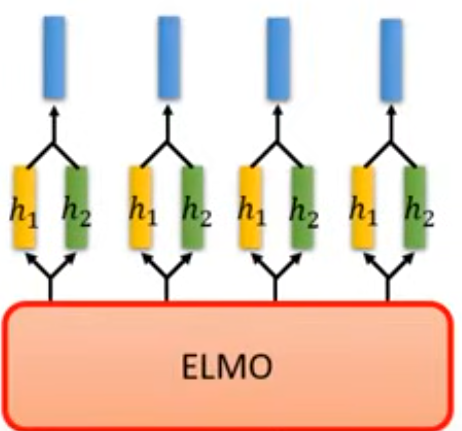
\includegraphics[width=\linewidth]{images/w6/ELMO.png}
		\caption{ELMO}
    \end{minipage}
    \hspace{4em}
    \begin{minipage}[t]{0.2 \linewidth}
        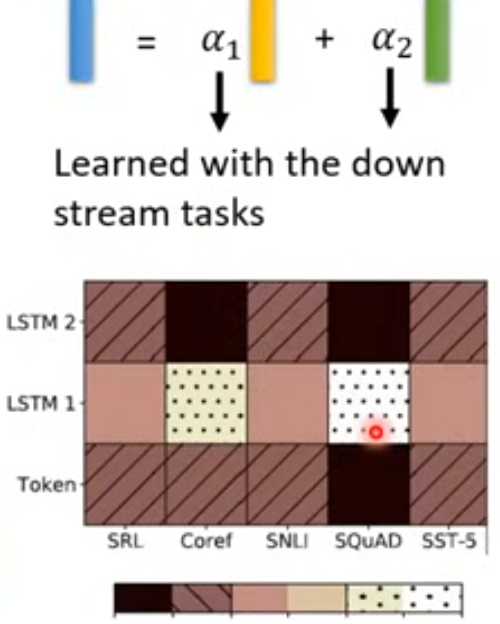
\includegraphics[width=\linewidth]{images/w6/weightedSum.png}
		\caption{權重學習}
    \end{minipage}
\end{figure}
\newpage

\section{BERT}
Bidirectional Encoder Representations from Transformers (BERT)是Transformer的Encoder (\autoref{fig:BERT-struct}左半部分)。

\begin{wrapfigure}[4]{r}{0.5\linewidth}
  \begin{center}
    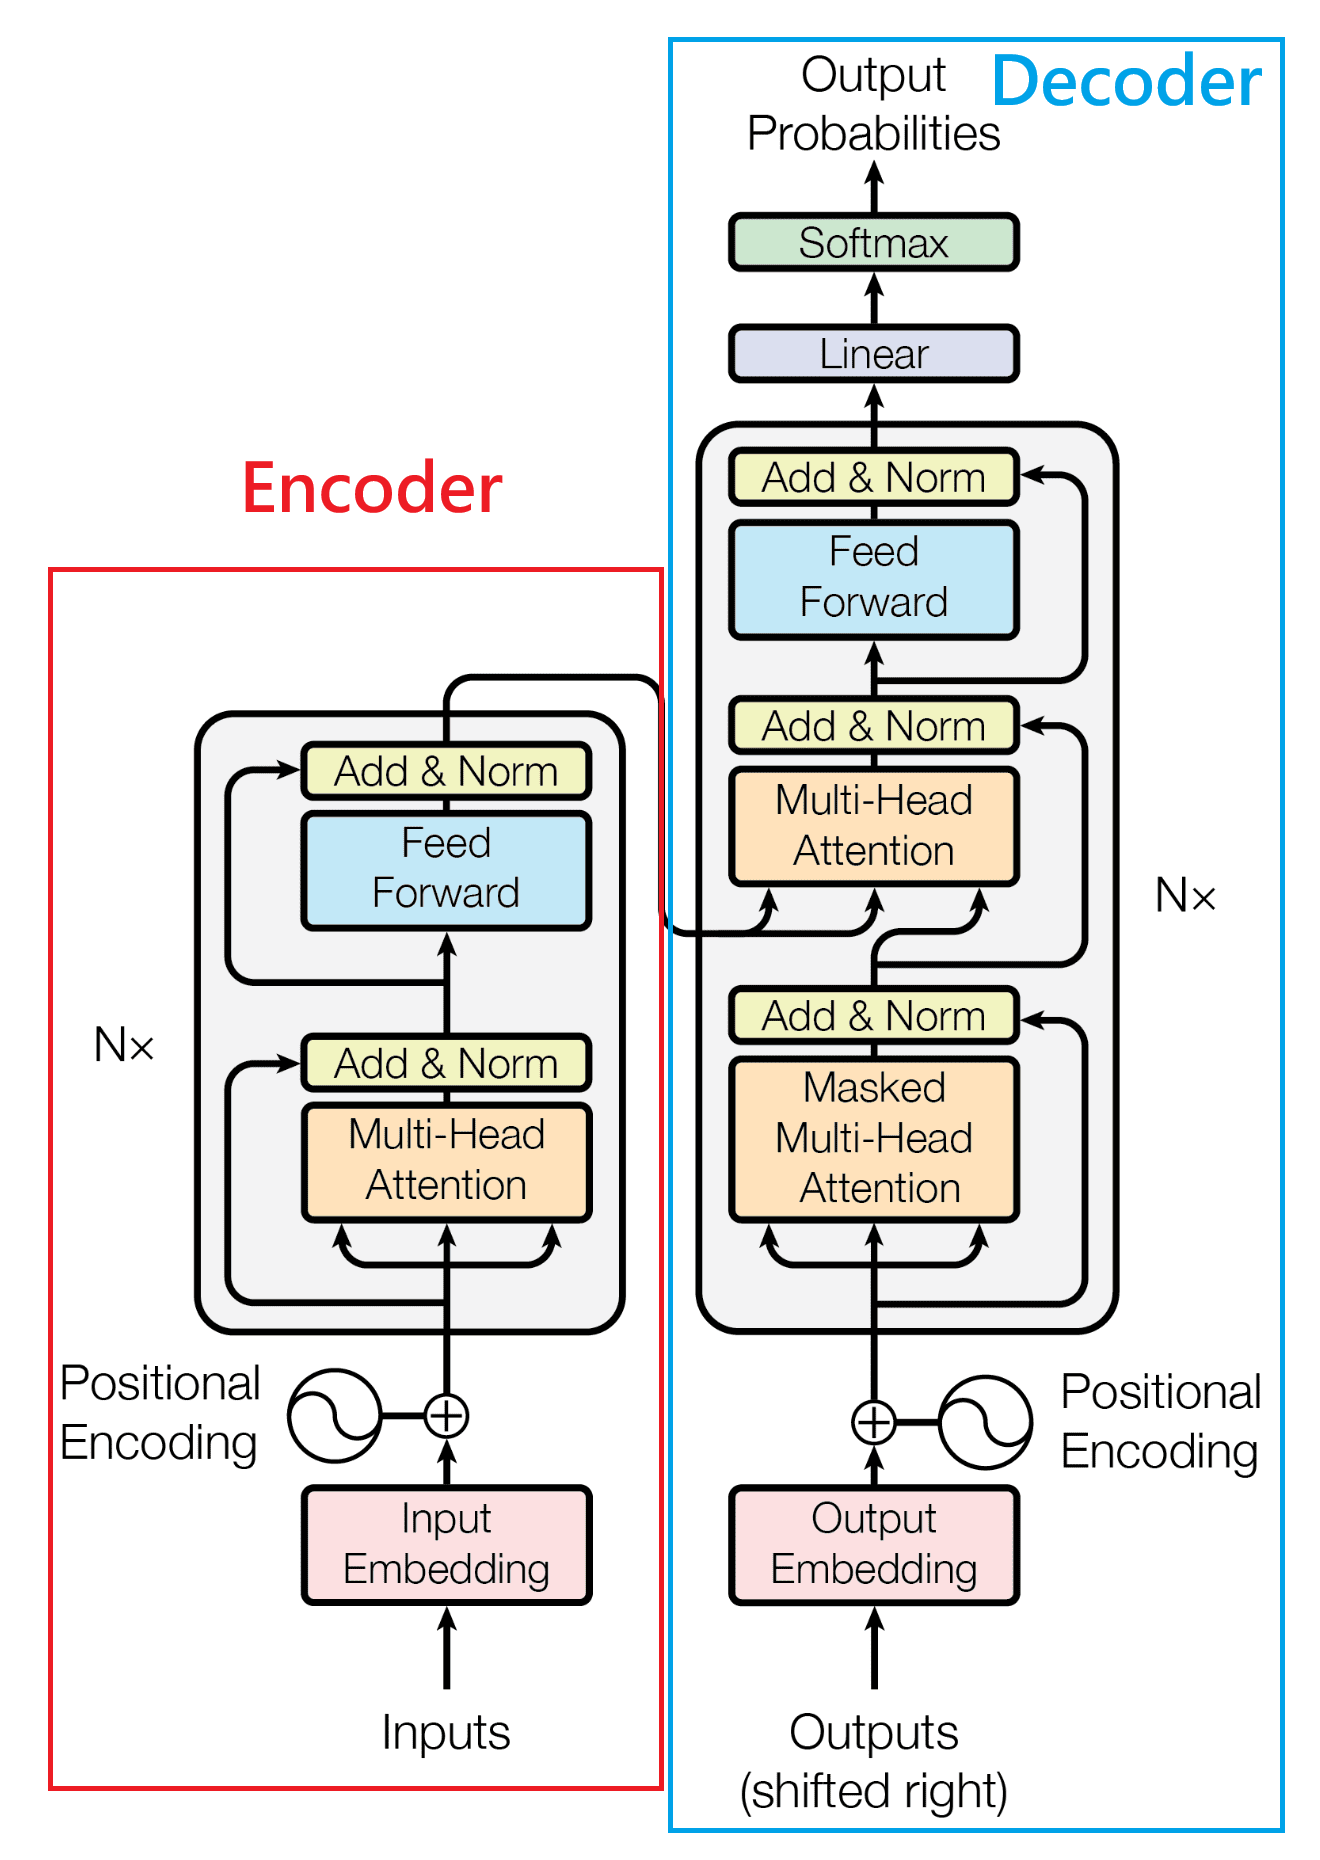
\includegraphics[width=0.4\textwidth]{images/w6/BERT_Struct.png}
  \end{center}
  \caption{BERT}
  \label{fig:BERT-struct}

  \vspace{3em}
 \makeatletter\def\@captype{table}\makeatother% "Change float to table"
    \caption{使用BERT的情況}
    \label{table:BERT-cases}
    \begin{tabular}{|l|l|l|l|}
    \hline
Case & Input                                               & Output             & Example      \\ \hline
1    & 一個句子                                                & class              & 文章分類         \\ \hline
2    & 一個句子                                                & class of each word & Slot filling \\ \hline
3    & 兩個句子                                                & class              & 自然語言推論       \\ \hline
4    & \begin{tabular}[c]{@{}l@{}}一篇文章\\ 一個問題\end{tabular} & 兩個整數               & SQuAD        \\ \hline
\end{tabular}

  \vspace{-\baselineskip}
\end{wrapfigure}

\subsection{訓練BERT}
\subsubsection{方法一:}
\textbf{Masked LM:} 把所有的句子內隨機15\%的詞彙換成叫做MASK的token,將MASK得到的embedding丟到Linear Multi-class Classifier讓他預測被MASK掉的詞彙是什麼。\\若兩個詞填在同一地方沒有違和感,那它們就\\有類似的embedding。
\subsubsection{方法二:}
\textbf{Next Sentence Prediction:} 給兩個句子BERT預測句子是否接再一起,需要給BERT兩個token分別是: [SEP](boundary of two sentences)和[CLS](position that outputs classification results)。\\
CLS通常是放在句子的開頭它代表要做分類,\\把CLS的embedding丟到Linear Binary Classifier\\來決定句子應不應該接再一起。

\subsection{使用BERT}
\textbf{Case 1:}輸入一個句子,輸出class \par
\textbf{Case 2:}輸入一個句子,輸出多個class  \par
\textbf{Case 3:} 輸入兩個句子,輸出class\par
\textbf{Case 4:} 給Model一篇文章和一個問題,輸出的兩個整數代表答案在那兩個整數間的token。\par

讓機器學習另外兩個vector,讓他們和文章中每個字的embedding做dot product,將算出來的值透過Softmax找到最高分。
\clearpage
\newpage

\begin{figure}[htbp!]
    \centering
    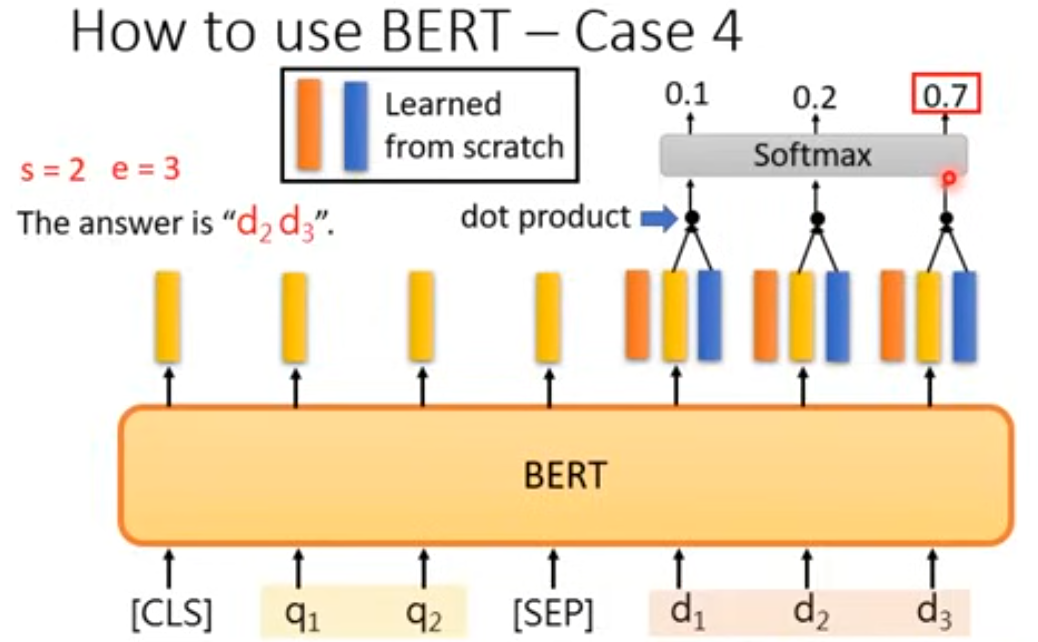
\includegraphics[width=0.5\linewidth]{images/w6/BERT-case4.png}
    \caption{BERT如何找出文章答案}
    \label{fig:BERT-case4}
\end{figure}

\section{GPT}
Generative Pre-Training(GPT)是一個超級大的語言模型,它的架構就是Transformer的Decoder,也就是\autoref{fig:BERT-struct}的右半邊。
\subsection{GPT可以做到的事情}
GPT可以做到在完全沒有相關的訓練資料下,做到閱讀理解、總結、翻譯。
\begin{figure}[htbp!]
    \centering
    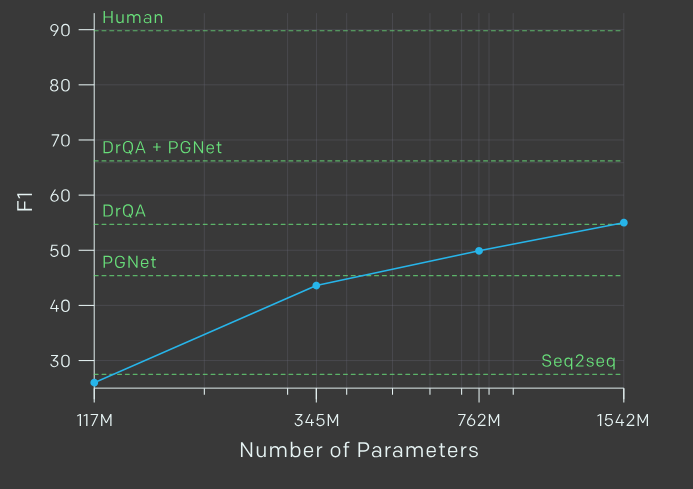
\includegraphics[width=0.5\linewidth]{images/w6/GPT2-reading.png}
    \caption{GPT-2閱讀理解的分數}
    \label{fig:GPT2-reading}
\end{figure}